 \documentclass{article}

% Language setting
% Replace `english' with e.g. `spanish' to change the document language
\usepackage[portuguese]{babel}

% Set page size and margins
% Replace `letterpaper' with `a4paper' for UK/EU standard size
\usepackage[letterpaper,top=2cm,bottom=2cm,left=3cm,right=3cm,marginparwidth=1.75cm]{geometry}

% Useful packages
\usepackage{amsmath}
\usepackage{graphicx}
\usepackage[colorlinks=true, allcolors=blue]{hyperref}
\usepackage{listings}
\usepackage{xcolor}

\definecolor{codegreen}{rgb}{0,0.6,0}
\definecolor{codegray}{rgb}{0.5,0.5,0.5}
\definecolor{codepurple}{rgb}{0.58,0,0.82}
\definecolor{backcolour}{rgb}{0.95,0.95,0.92}

\lstdefinestyle{mystyle}{
    backgroundcolor=\color{backcolour},   
    commentstyle=\color{codegreen},
    keywordstyle=\color{magenta},
    numberstyle=\tiny\color{codegray},
    stringstyle=\color{codepurple},
    basicstyle=\ttfamily\footnotesize,
    breakatwhitespace=false,         
    breaklines=true,                 
    captionpos=b,                    
    keepspaces=true,                 
    numbers=left,                    
    numbersep=5pt,                  
    showspaces=false,                
    showstringspaces=false,
    showtabs=false,                  
    tabsize=2
}

\lstset{style=mystyle}

\title{TP2 - Redes de Computadores}
\author{Francisco Ferreira - a100660\\Júlio Pinto - a100742\\Rui Lopes - a100643}

\begin{document}
\maketitle
\tableofcontents

\pagebreak
\bigskip

\section{Parte I - Exercício 1}

Prepare uma topologia CORE para verificar o comportamento do traceroute. Na topologia deve existir: um host (pc) cliente
designado Lost, cujo router de acesso é RA1; o router RA1 está simultaneamente ligado a dois routers no core da rede RC1 e RC2;
estes estão conectados a um router de acesso RA2, que por sua vez, se liga a um host (servidor) designado Found. Ajuste o nome
dos equipamentos atribuídos por defeito para o enunciado. Apenas nas ligações (links) da rede de core, estabeleça um tempo de
propagação de 15 ms. Após ativar a topologia, note que pode não existir conectividade IP imediata entre Lost e Found até que o
anúncio de rotas entre routers estabilize.


\begin{figure}[h]
    \centering
    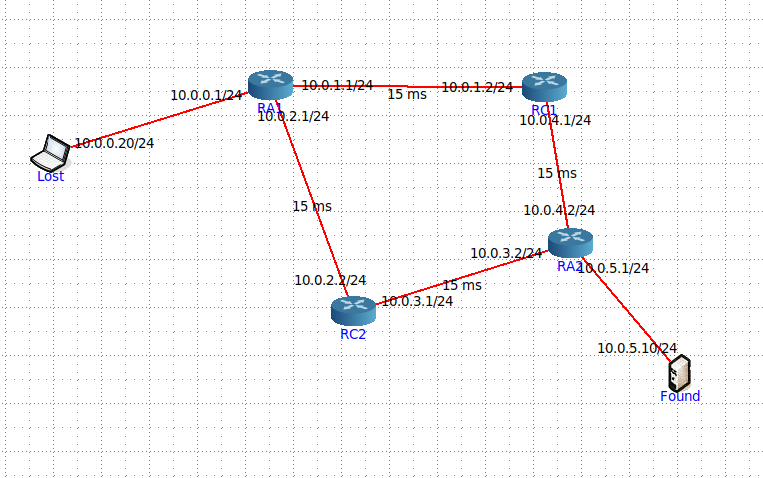
\includegraphics[width=\textwidth]{top1a.png}
    \caption{Topologia do exercício 1}
\end{figure}

\subsection{Alínea a)}

Active o Wireshark no host Lost. Numa shell de Lost execute o comando traceroute -I para o endereço IP do
Found. Registe e analise o tráfego ICMP enviado pelo sistema Lost e o tráfego ICMP recebido como resposta.
Explique os resultados obtidos tendo em conta o princípio de funcionamento do traceroute.



\subsubsection{Resposta alínea a)}

O comando \emph{traceroute} é usado para rastrear o caminho que um pacote de rede leva de um host de origem para uma host destino. Ele faz isso enviando pacotes ICMP com diferentes valores TTL para o host destino (neste caso, Found). O TTL é um valor numérico no header do pacote IP que indica quantos routers o pacote pode passar antes de ser descartado. Quando um pacote alcança um router, o router decrementa o valor TTL e encaminha o pacote para o próximo router no caminho para o Found.

O primeiro pacote enviado tem um TTL inicial de 1. O primeiro router no caminho para o Found recebe o pacote e descarta-o, e envia de volta uma mensagem ICMP de "time exceeded", indicando que o TTL do pacote expirou antes que o pacote pudesse alcançar o Found. O \emph{traceroute} regista o endereço IP do primeiro router e o tempo que levou para receber a mensagem ICMP de "time exceeded". Em seguida, o traceroute envia outro pacote ICMP com um TTL de 2, que fará com que ele passe por dois routers antes de expirar e receber outra mensagem ICMP de "time exceeded". O processo continua com incrementos no valor do TTL até que o Found seja alcançado e responda com uma mensagem ICMP de "echo reply".

Ao observar o tráfego gerado pelo traceroute com o Wireshark, é possível visualizar as mensagens ICMP de "time exceeded" enviadas pelos routers ao longo do caminho e as mensagens ICMP de "echo reply" enviadas pelo Found. Isso permite que se tenha uma ideia do caminho que os pacotes estão a tomar para alcançar o Found e o tempo que leva para cada pacote alcançar o próximo router.

\bigskip

\begin{lstlisting}[language=Bash]
> traceroute -I 10.0.5.10   
traceroute to 10.0.5.10 (10.0.5.10), 30 hops max, 60 byte packets
 1  10.0.0.1 (10.0.0.1)  0.175 ms  0.039 ms  0.031 ms
 2  10.0.1.2 (10.0.1.2)  30.832 ms  30.713 ms  30.689 ms
 3  10.0.3.2 (10.0.3.2)  94.447 ms  94.435 ms  94.423 ms
 4  10.0.5.10 (10.0.5.10)  94.408 ms  94.395 ms  94.383 ms 
\end{lstlisting}

\subsection{Alínea b)}

Qual deve ser o valor inicial mínimo do campo TTL para alcançar o servidor Found? Verifique na prática que a
sua resposta está correta.

\subsubsection{Resposta alínea b)}

O valor mínimo do TTL deve ser 4, isto pois, é a essa distância que se encontra o host \emph{Found}.
Como se pode comprovar através da análise da imagem anexada.

\begin{figure}[h]
    \centering
    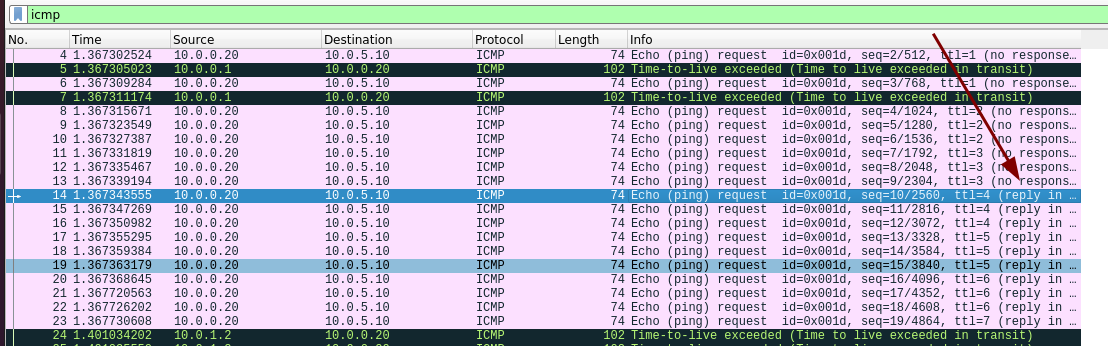
\includegraphics[width=\textwidth]{image2.png}
\end{figure}

\pagebreak

\subsection{Alínea c)}
Calcule o valor médio do tempo de ida-e-volta (RTT - Round-Trip Time) obtido no acesso ao servidor. Por modo
a obter uma média mais confiável, poderá alterar o número pacotes de prova com a opção -q.

\subsubsection{Resposta alínea c)}

Calculando a média a partir da última linha do \emph{traceroute}, deduzimos que o \emph{Round-Trip Time} tem o valor de:
\[ RTT = (62.691 + 61.266 + 61.238 + 61.224 + 61.212) / 5 = 61.5262 ms \]

\begin{lstlisting}[language=Bash]
> traceroute -I 10.0.5.10 -q 5                                             
traceroute to 10.0.5.10 (10.0.5.10), 30 hops max, 60 byte packets
 1  10.0.0.1 (10.0.0.1)  0.066 ms  0.021 ms  0.017 ms  0.017 ms  0.019 ms
 2  10.0.1.2 (10.0.1.2)  30.268 ms  30.250 ms  30.237 ms  31.318 ms  31.306 ms
 3  10.0.3.2 (10.0.3.2)  62.758 ms  62.745 ms  62.732 ms  62.720 ms  62.707 ms
 4  10.0.5.10 (10.0.5.10)  62.691 ms  61.266 ms  61.238 ms  61.224 ms  61.212 ms
\end{lstlisting}

\subsection{Alínea d)}

O valor médio do atraso num sentido (One-Way Delay) poderia ser calculado com precisão dividindo o RTT por
dois? O que torna difícil o cálculo desta métrica numa rede real?

\subsubsection{Resposta alínea d)}

Não, o valor médio do atraso num sentido (One-Way Delay) não pode ser calculado simplesmente dividindo o RTT por dois. Isto acontece porque o RTT inclui o tempo de ida e volta, enquanto o One-Way Delay mede apenas o tempo de atraso num único sentido.

Para medir o One-Way Delay, é necessário ter uma fonte confiável de tempo para sincronizar os relógios de todos os dispositivos envolvidos na comunicação. Além disso, é preciso ter um método para registar a hora em que um pacote é enviado e recebido em cada dispositivo. A partir dessas informações, é possível calcular o atraso em cada sentido.

No entanto, o cálculo do One-Way Delay numa rede real pode ser difícil porque a rede pode ter um comportamento imprevisível e variável. Por exemplo, o atraso pode variar devido a congestionamento da rede, problemas de encaminhamento, problemas de configuração de rede, entre outros fatores. Além disso, pode haver dispositivos intermédios, como switches e routers, que introduzem atrasos adicionais na comunicação. Portanto, é importante usar técnicas avançadas de medição e monitorização da rede para medir o One-Way Delay com precisão numa rede real.

\pagebreak 
 
\section{Parte I - Exercício 2}
Usando o wireshark capture o tráfego gerado pelo traceroute sem especificar o tamanho do pacote, i.e., quando é usado o tamanho
do pacote de prova por defeito. Utilize como máquina destino o host marco.uminho.pt. Pare a captura. Com base no tráfego
capturado, identifique os pedidos ICMP Echo Request e o conjunto de mensagens devolvidas como resposta.

Selecione a primeira mensagem ICMP capturada e centre a análise no nível protocolar IP e, em particular, do cabeçalho IP
(expanda o tab correspondente na janela de detalhe do wireshark).

\bigskip
\subsection{Alínea a)}

Qual é o endereço IP da interface ativa do seu computador?

\subsubsection{Resposta alínea a)}

O endereço IP da interface ativa do computador é 172.26.44.37

\subsection{Alínea b)}

Qual é o valor do campo protocol? O que permite identificar?

\subsubsection{Resposta alínea b)}

O valor do campo protolocol é ICMP(1). Este campo permite identificar que o datagrama IP contém uma mensagem ICMP.

\subsection{Alínea c)}

Quantos bytes tem o cabeçalho IPv4? Quantos bytes tem o campo de dados (payload) do datagrama? Como se
calcula o tamanho do payload?

\subsubsection{Resposta alínea c)}

O cabeçalho IPv4 tem 20 bytes. Enquanto que o \emph{Payload} do datagrama tem 40 bytes.
\\
Payload = total length - header length
\\
Payload = 60 - 20 = 40 bytes

\subsection{Alínea d)}

O datagrama IP foi fragmentado? Justifique.

\subsubsection{Resposta alínea d)}

Não. Concluímos que o datagram não foi fragmentado isto pois a flag \emph{"More Fragments"} não contém nenhum valor e o \emph{"Fragment Offset"} é igual a 0.

\pagebreak
\begin{figure}[h]
    \centering
    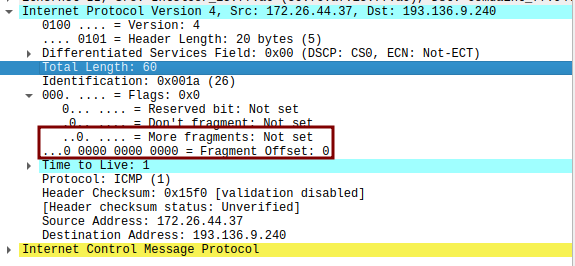
\includegraphics[width=\textwidth]{image3.png}
    \caption{Base da resposta da alínea d)}
\end{figure}

\subsection{Alínea e)}

 Ordene os pacotes capturados de acordo com o endereço IP fonte (e.g., selecionando o cabeçalho da coluna
Source), e analise a sequência de tráfego ICMP gerado a partir do endereço IP atribuído à interface da sua
máquina. Para a sequência de mensagens ICMP enviadas pelo seu computador, indique que campos do
cabeçalho IP variam de pacote para pacote.

\subsubsection{Resposta alínea e)}

Os campos que sofrem alterações são: o campo de identificação, o TTL (varia apenas de três em três pacotes) e o "Header Checksum".


\subsection{Alínea f)}

Observa algum padrão nos valores do campo de Identificação do datagrama IP e TTL?

\subsubsection{Resposta alínea f)}

O valor do campo de identificação sobre sempre uma unidade em hexadecimal. Já o TTL sobe em uma unidade a cada três pacotes enviados pela minha máquina. 

\subsection{Alínea g)}

Ordene o tráfego capturado por endereço destino e encontre a série de respostas ICMP TTL Exceeded enviadas
ao seu computador.

i. Qual é o valor do campo TTL recebido no seu computador? Esse valor permanece constante para todas
as mensagens de resposta ICMP TTL Exceeded recebidas no seu computador? Porquê?

ii. Porque razão as mensagens de resposta ICMP TTL Exceeded são sempre enviadas na origem com um
valor TTL relativamente alto?

\subsubsection{Resposta alínea g.i)}
O valor recebido varia entre 253 e 255, portanto, nem sempre é constante. De forma a garantir que o pacote é reencaminhado com sucesso, usa-se sempre o maior valor possível associado ao TTL. Uma vez que só temos 8 bits disponíveis, o valor máximo é 256  \((2^8)\), mas como já foi efetuado um salto o valor passa a ser 255. Além disso, os valores variarem entre 253 e 255 deve-se ao facto do TTL ser decrementado no caminho de volta e os nós estarem a distâncias diferentes do destino.

\subsubsection{Resposta alínea g.ii)}
Como dito anteriormente, para garantir que o pacote é reencaminhado com sucesso.

\subsection{Alínea h)}

Sabendo que o ICMP é um protocolo pertencente ao nível de rede, discuta se a informação contida no cabeçalho
ICMP poderia ser incluída no cabeçalho IPv4? Quais seriam as vantagens/desvantagens resultantes dessa
hipotética inclusão?

\subsubsection{Resposta alínea h)}

Sim, teoricamente, a informação contida no cabeçalho ICMP poderia ser incluída no cabeçalho IPv4.
Uma das principais vantagens de incluir as informações do ICMP no cabeçalho IPv4 é que isso pode reduzir o tamanho dos pacotes enviados pela rede, já que a sobrecarga adicional de um cabeçalho ICMP separado seria eliminada. Isso pode ser especialmente benéfico em redes onde a largura de banda é limitada e cada byte de dados é valioso.
Embora seja possível incluir as informações do ICMP no cabeçalho IPv4, essa abordagem pode ter algumas desvantagens significativas, incluindo aumento da complexidade, problemas de compatibilidade e sobrecarga desnecessária do cabeçalho IPv4.

\pagebreak

\section{Parte I - Exercício 3}

Pretende-se agora analisar a fragmentação de pacotes IP. Usando o wireshark, capture e observe o tráfego gerado depois do
tamanho de pacote ter sido definido para (3500 + X) bytes, em que X é o número do grupo de trabalho (e.g., X=22 para o grupo
PL22).

\subsection{Alínea a)}

Localize a primeira mensagem ICMP. Porque é que houve necessidade de fragmentar o pacote inicial?

\subsubsection{Resposta alínea a)}

O valor máximo que um datagrama ICMP pode ter é de 1500 bytes, onde 1480 bytes são para os dados e 20 bytes são para o cabeçalho. Uma vez que os pacotes enviados têm um tamanho igual a 3512 bytes, foi necessário recorrer a fragmentação.

\subsection{Alínea b)}

Imprima o primeiro fragmento do datagrama IP original. Que informação no cabeçalho indica que o datagrama foi
fragmentado? Que informação no cabeçalho IP indica que se trata do primeiro fragmento? Qual é o tamanho
deste datagrama IP?

\subsubsection{Resposta alínea b)}

Uma vez que a flag "More fragments" tem o valor 1, é possível afirmar que o datagrama foi fragmentado. Além disso, como o "Fragment offset" tem o valor 0, isso significa que este fragmento se trata do primeiro. O tamanho do datagrama é de 1480 bytes, valor coincidente com a capacidade máxima de dados num datagrama ICMP.

\subsection{Alínea c)}

Imprima o segundo fragmento do datagrama IP original. Que informação do cabeçalho IP indica que não se trata
do 1º fragmento? Existem mais fragmentos? O que nos permite afirmar isso?

\subsubsection{Resposta alínea c)}

É possível afirmar que este fragmento não se trata do primeiro, pois o "Fragment offset" é diferente de 0. Neste caso, o "Fragment offset" é de 1480. Isto pois, o fragmento anterior tinha tamanho igual a 1480 bytes (como anteriormente foi referido). No entanto, existem mais fragmentos do datagrama IP original, pois a flag "More fragments" tem o valor 1.

\subsection{Alínea d)}

Estime teoricamente o número de fragmentos gerados a partir do datagrama IP original e o número de bytes
transportados no último fragmento desse datagrama. Compare os dois valores estimados com os obtidos através
do wireshark.
\pagebreak
\subsubsection{Resposta alínea d)}

Tendo por base um datagrama IP com 3512 bytes de dados e a MTU (maximum transmission unit) igual a 1500, irão ser gerados 3 fragmentos. Os dois primeiros fragmentos terão 1500 bytes (1480 bytes de dados cada) e o último 572 (552 bytes de dados), totalizando então 3512 bytes de dados.
No entanto, em cada um dos dois primeiros pacotes, apenas 1480 bytes irão ser de dados. Isto deve-se ao facto de 20 bytes estarem reservados para o cabeçalho IP. No último caso, aplica-se também o raciocínio de 20 bytes estarem reservados para o cabeçalho IP, mas apenas 552 bytes irão ser de dados.
Segundo o wireshark, foram também gerados 3 fragmentos, o que bate certo com o estimado teoricamente. O tamanho de cada fragmento, ao nível dos dados, foi também o esperado: 1480 + 1480 + 552

\begin{figure}[h]
    \centering
    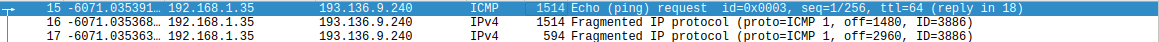
\includegraphics[width=\textwidth]{image4.png}
\end{figure}

\subsection{Alínea e)}

Como se deteta o último fragmento correspondente ao datagrama original? Estabeleça um filtro no Wireshark que
permita listar o último fragmento do primeiro datagrama IP segmentado.

\subsubsection{Resposta alínea e)}

O último fragmento tem sempre a flag "More fragments" igual a 0 e o "Fragment offset" diferente de 0. Filtro para o wireshark:
\begin{lstlisting}[language=Bash]
> ip.dst == 193.136.9.240 && ip.flags.mf == 0 && ip.frag_offset > 0 && ip.id == 0x3886
\end{lstlisting}

\begin{figure}[h]
    \centering
    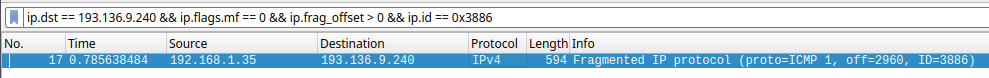
\includegraphics[width=\textwidth]{image5.png}
\end{figure}


\subsection{Alínea f)}

Identifique o equipamento onde o datagrama IP original é reconstruído a partir dos fragmentos. A reconstrução
poderia ter ocorrido noutro equipamento diferente do identificado? Porquê?

\subsubsection{Resposta alínea f)}

O pacote é refragmentado no equipamanto destino (identificado pelo ip 193.136.9.240). Sim, a reconstrução poderia ter ocorrido noutro equipamento - desde que para isso, esse equipamento tivesse acesso a todos os fragmentos. No entanto, os equipamentos intermédios apenas reencaminham tráfego (sem olhar para os seus conteúdos).

\subsection{Alínea g)}

Indique, resumindo, os campos que mudam no cabeçalho IP entre os diferentes fragmentos, e explique a forma
como essa informação permite reconstruir o datagrama original.

\subsubsection{Resposta alínea g)}

Os campos que sofrem alteração são: a flag "More fragments", que tem o valor 1 em todos os fragmentos exceto o último; o "Fragment offset", que indica a posição inicial dos dados no fragmento atual, em relação à posição inicial de dados no pacote original. Este "offset" é utilizado, depois, para reagrupar os fragmentos. Além disso, o "Header checksum" também sofre alterações, já que cada fragmento possui o seu próprio cabeçalho e é necessário garantir a integridade de cada um deles.

\subsection{Alínea h)}

Por que razão apenas o primeiro fragmento de cada pacote é identificado como sendo um pacote ICMP?

\subsubsection{Resposta alínea h)}

Ao transmitir um pacote ICMP, esta conta com um cabeçalho ICMP, que se encontra no início da pacote. No entanto, quando o pacote é fragmentado, apenas o primeiro é identificado como ICMP, pois esse é que o "leva" o cabeçalho ICMP consigo (todos os outros "levam" cabeçalhos IP).

\subsection{Alínea i)}

Com que valor é o tamanho do datagrama comparado a fim de se determinar se este deve ser fragmentado?
Quais seriam os efeitos na rede ao aumentar/diminuir este valor?

\subsubsection{Resposta alínea i)}
O datagrama é comparado com o valor 1500, o MTU (Maximum Transmission Unit, neste caso). A variação deste valor influencia a quantidade de fragmentos em que o pacote tem de ser transmitido. Quanto maior este valor, menos fragmentos serão necessários.

\subsection{Alínea j)}

Sabendo que no comando ping a opção -f (Windows), -M do (Linux) ou –D (Mac) ativa a flag “Don’t Fragment”
(DF) no cabeçalho do IPv4, usando ping <opção DF> <opção pkt\_size> SIZE marco.uminho.pt, (opção pkt\_size
= –l (Windows) ou –s (Linux, Mac), determine o valor máximo de SIZE sem que ocorra fragmentação do pacote?
Justifique o valor obtido.

\subsubsection{Resposta alínea j)}
O tamanho máximo de SIZE é de 1472. Após este valor (1473 ou mais), ocorre fragmentação. Isto deve-se ao facto do MTU ser 1500, mas existirem 20 bytes alocados para o cabeçalho IP e 8 bytes alocados para o cabeçalho ICMP. É possível demonstrar isso atráves da imagem abaixo:
\begin{figure}[h]
    \centering
    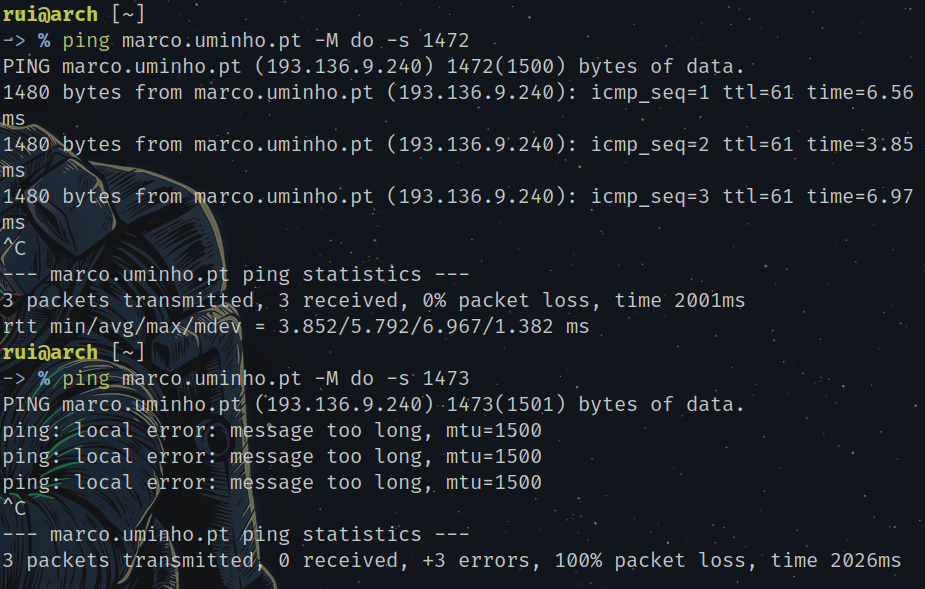
\includegraphics[width=\textwidth]{image6.png}
\end{figure}

\pagebreak

\section{Parte II - Exercício 1}

D.Afonso Henriques afirma ter problemas de comunicação com a sua mãe, D.Teresa. Este alega que o problema
deverá estar no dispositivo de D.Teresa, uma vez que no dia anterior conseguiu enviar a sua declaração do IRS para
o portal das finanças, e não tem qualquer problema em ver as suas séries favoritas disponíveis na rede de conteúdos

\subsection{Alínea a)}

Averigue, através do comando ping, que AfonsoHenriques tem efetivamente conectividade com o servidor Financas e com os servidores da CDN.

\subsubsection{Resposta alínea a)}

De maneira a concluir que, efetivamente, AfonsoHenriques tem conectividade com o servidor Finanças e os servidores da CDN recolhemos as seguintes imagens:
\begin{figure}[h]
    \centering
    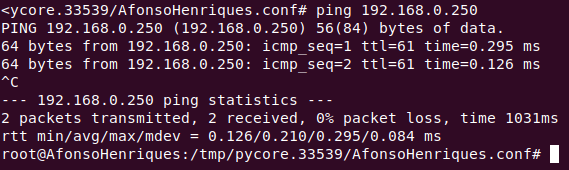
\includegraphics[scale=0.5]{financas.png}
    \caption{Conectividade ao Servidor Finanças.}
\end{figure}
\begin{figure}[h]
    \centering
    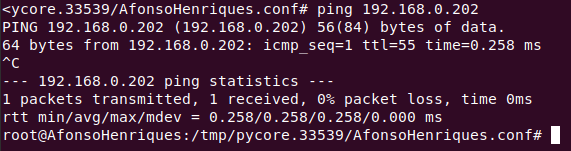
\includegraphics[scale=0.5]{cdn1.png}
    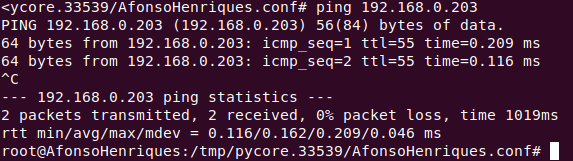
\includegraphics[scale=0.5]{cdn2.png}
    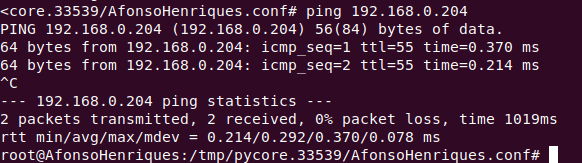
\includegraphics[scale=0.5]{cdn3.png}
    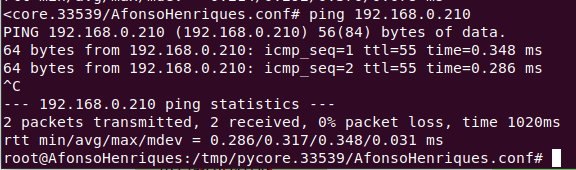
\includegraphics[scale=0.5]{cdn4.png}
    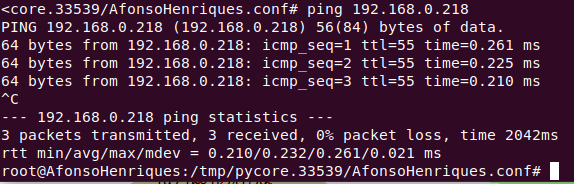
\includegraphics[scale=0.5]{cdn5.png}
    \caption{Conectividade aos hosts do CDN.}
\end{figure}
\pagebreak

\subsection{Alínea b)}

Recorrendo ao comando netstat -rn, analise as tabelas de encaminhamento dos dispositivos
AfonsoHenriques e Teresa. Existe algum problema com as suas entradas? Identifique e descreva a utilidade
de cada uma das entradas destes dois hosts

\subsubsection{Resposta alínea b)}

Tabela de reencaminhamento de AfonsoHenriques:
\begin{lstlisting}[language=Bash]
> netstat -rn
Kernel IP routing table
Destination     Gateway         Genmask         Flags   MSS Window  irtt Iface
0.0.0.0         192.168.0.225   0.0.0.0         UG        0 0          0 eth0
192.168.0.224   0.0.0.0         255.255.255.248 U         0 0          0 eth0
\end{lstlisting}
Esta tabela não apresenta nenhum problema com as entradas. A primeira entrada é a "default", ou seja, todo o tráfego cujo IP destino não esteja discriminado na tabela é reencaminhado por aí. A segunda entrada refere-se a todos os IPs que se encontrem na mesma subrede que o equipamento atual. Nesses casos, o tráfego é reencaminhado pelo próprio equipamento até ao host destino.
\pagebreak

Tabela de reencaminhamento de Teresa:
\begin{lstlisting}[language=Bash]
> netstat -rn
Kernel IP routing table
Destination     Gateway         Genmask         Flags   MSS Window  irtt Iface
0.0.0.0         192.168.0.193   0.0.0.0         UG        0 0          0 eth0
192.168.0.192   0.0.0.0         255.255.255.248 U         0 0          0 eth0
\end{lstlisting}

Conseguimos deduzir que o foi dito sobre a tabela anterior também poderá ser dito relativamente a esta tabela. A única diferença seriam os seus endereços IP.

\subsection{Alínea c)}
Utilize o Wireshark para investigar o comportamento dos routers do core da rede (n1 a n6) quando tenta
estabelecer comunicação entre os hosts AfonsoHenriques e Teresa. Indique que dispositivo(s) não
permite(m) o encaminhamento correto dos pacotes. Seguidamente, avalie e explique a(s) causa(s) do
funcionamento incorreto do dispositivo.
Utilize o comando ip route add/del para adicionar as rotas necessárias ou remover rotas incorretas. Verifique
a sintaxe completa do comando a usar com man ip-route ou man route. Poderá também utilizar o comando
traceroute para se certificar do caminho nó a nó. Considere a alínea resolvida assim que houver tráfego a
chegar ao ISP CondadOnline.

\subsubsection{Resposta alínea c)}
\begin{lstlisting}
> traceroute 192.168.0.194                           
traceroute to 192.168.0.194 (192.168.0.194), 30 hops max, 60 byte packets
 1  192.168.0.225 (192.168.0.225)  0.175 ms  0.028 ms  0.035 ms
 2  172.16.143.1 (172.16.143.1)  0.090 ms  0.030 ms  0.028 ms
 3  10.0.0.29 (10.0.0.29)  0.086 ms !N  0.038 ms !N *
\end{lstlisting}
Executando o comando traceroute 192.168.0.194 é possível perceber que o problema está no "n5", identificado pelo IP 10.0.029.

Utilizando o comando netstat -rn nesse mesmo host, é possível perceber que não existe uma rota para encaminhar tráfego com destino a IPs 192.168.0.192/29:
\begin{lstlisting}
> netstat -rn
Kernel IP routing table
Destination     Gateway         Genmask         Flags   MSS Window  irtt Iface
10.0.0.0        10.0.0.25       255.255.255.252 UG        0 0          0 eth1
10.0.0.4        10.0.0.25       255.255.255.252 UG        0 0          0 eth1
10.0.0.8        10.0.0.25       255.255.255.252 UG        0 0          0 eth1
10.0.0.12       10.0.0.25       255.255.255.252 UG        0 0          0 eth1
10.0.0.16       10.0.0.25       255.255.255.252 UG        0 0          0 eth1
10.0.0.20       10.0.0.25       255.255.255.252 UG        0 0          0 eth1
10.0.0.24       0.0.0.0         255.255.255.252 U         0 0          0 eth1
10.0.0.28       0.0.0.0         255.255.255.252 U         0 0          0 eth0
172.0.0.0       10.0.0.30       255.0.0.0       UG        0 0          0 eth0
172.16.142.0    10.0.0.25       255.255.255.248 UG        0 0          0 eth1
172.16.143.0    10.0.0.30       255.255.255.252 UG        0 0          0 eth0
172.16.143.0    10.0.0.30       255.255.255.248 UG        0 0          0 eth0
172.16.143.4    10.0.0.30       255.255.255.252 UG        0 0          0 eth0
192.142.0.4     10.0.0.25       255.255.255.252 UG        0 0          0 eth1
192.168.0.200   10.0.0.25       255.255.255.248 UG        0 0          0 eth1
192.168.0.208   10.0.0.25       255.255.255.248 UG        0 0          0 eth1
192.168.0.216   10.0.0.25       255.255.255.248 UG        0 0          0 eth1
192.168.0.224   10.0.0.30       255.255.255.248 UG        0 0          0 eth0
192.168.0.232   10.0.0.30       255.255.255.248 UG        0 0          0 eth0
192.168.0.240   10.0.0.30       255.255.255.248 UG        0 0          0 eth0
192.168.0.248   10.0.0.30       255.255.255.248 UG        0 0          0 eth0
\end{lstlisting}
Devemos, assim, adicionar essa rota com o comando: ip route add 192.168.0.192/29 via 10.0.0.25

No entanto, o problema de comunicação entre AfonsoHenriques e Teresa mantém-se, tal como é possível inferir através do seguinte comando:

\begin{lstlisting}
> traceroute 192.168.0.194                  
traceroute to 192.168.0.194 (192.168.0.194), 30 hops max, 60 byte packets
 1  192.168.0.225 (192.168.0.225)  0.061 ms  0.037 ms  0.015 ms
 2  172.16.143.1 (172.16.143.1)  0.035 ms  0.024 ms  0.023 ms
 3  10.0.0.29 (10.0.0.29)  0.045 ms  0.032 ms  0.032 ms
 4  10.0.0.25 (10.0.0.25)  0.052 ms  0.041 ms  0.040 ms
 5  10.0.0.25 (10.0.0.25)  3055.726 ms !H  3055.655 ms !H  3055.602 ms !H
\end{lstlisting}
Agora o problema encontra-se no "n2". Acontece que a rota 192.168.0.194/31 dá match em vez da rota 192.168.0.192/29. Isto deve-se à forma como o match se dá, usando "Longest prefix match". Para resolver o problema é só remover a entrada 192.168.0.194/31 com o comando ip route del 192.168.0.194/31

No entanto, permanecemos ainda com outro problema. O tráfego encaminhado pelo "n2" para o "n1" é novamente reencaminhado para o "n2". Criando um loop de reencaminhamentos, que termina quando o TTL dos pacotes é igual a 0. Para isso, é necessário alterar a forma como o "n1" encaminha o tráfego com destino a Teresa. 
Em baixo, está a tabela de encaminhamento do "n1": 
\begin{lstlisting}
> netstat -rn
Kernel IP routing table
Destination     Gateway         Genmask         Flags   MSS Window  irtt Iface
10.0.0.0        10.0.0.9        255.255.255.252 UG        0 0          0 eth0
10.0.0.4        10.0.0.9        255.255.255.252 UG        0 0          0 eth0
10.0.0.8        0.0.0.0         255.255.255.252 U         0 0          0 eth0
10.0.0.12       0.0.0.0         255.255.255.252 U         0 0          0 eth1
10.0.0.16       10.0.0.9        255.255.255.252 UG        0 0          0 eth0
10.0.0.20       10.0.0.14       255.255.255.252 UG        0 0          0 eth1
10.0.0.24       10.0.0.14       255.255.255.252 UG        0 0          0 eth1
10.0.0.28       10.0.0.14       255.255.255.252 UG        0 0          0 eth1
172.0.0.0       10.0.0.14       255.0.0.0       UG        0 0          0 eth1
172.16.142.0    10.0.0.9        255.255.255.252 UG        0 0          0 eth0
172.16.142.4    10.0.0.9        255.255.255.252 UG        0 0          0 eth0
172.16.143.0    10.0.0.14       255.255.255.252 UG        0 0          0 eth1
172.16.143.4    10.0.0.14       255.255.255.252 UG        0 0          0 eth1
192.168.0.192   10.0.0.14       255.255.255.248 UG        0 0          0 eth1
192.168.0.200   10.0.0.9        255.255.255.248 UG        0 0          0 eth0
192.168.0.208   10.0.0.9        255.255.255.248 UG        0 0          0 eth0
192.168.0.216   10.0.0.9        255.255.255.248 UG        0 0          0 eth0
192.168.0.224   10.0.0.14       255.255.255.248 UG        0 0          0 eth1
192.168.0.232   10.0.0.14       255.255.255.248 UG        0 0          0 eth1
192.168.0.240   10.0.0.14       255.255.255.248 UG        0 0          0 eth1
192.168.0.248   10.0.0.14       255.255.255.248 UG        0 0          0 eth1
\end{lstlisting}
É possível perceber através da linha 17, que o tráfego é reencaminhado novamente para o "n2"

Portanto, basta alterar esta entrada e definir o Gateway para o "n3". Executando os seguintes comandos: 
\begin{lstlisting}
> ip route del 192.168.0.192/29
> ip route add 192.168.0.192/29 via 10.0.0.9
\end{lstlisting}

Após isto, no caminho para a Teresa, o pacote já consegue chegar ao CondadOnline.

\subsection{Alínea d)}

Uma vez que o core da rede esteja a encaminhar corretamente os pacotes enviados por AfonsoHenriques,
confira com o Wireshark se estes são recebidos por Teresa.
\bigskip

i) Em caso afirmativo, porque é que continua a não existir conectividade entre D.Teresa e D.Afonso
Henriques? Efetue as alterações necessárias para garantir que a conectividade é restabelecida e o confronto
entre os dois é evitado.

ii) As rotas dos pacotes ICMP echo reply são as mesmas, mas em sentido inverso, que as rotas dos pacotes
ICMP echo request enviados entre AfonsoHenriques e Teresa? (Sugestão: analise as rotas nos dois sentidos
com o traceroute). Mostre graficamente a rota seguida nos dois sentidos por esses pacotes ICMP.

\subsubsection{Resposta alínea d.i)}
É possível constatar, executando o comando traceroute 192.168.0.194, que, a partir, do CondadOnline não existiu uma resposta de volta.
\begin{lstlisting}
> traceroute 192.168.0.194                  
traceroute to 192.168.0.194 (192.168.0.194), 30 hops max, 60 byte packets
 1  192.168.0.225 (192.168.0.225)  0.073 ms  0.021 ms  0.017 ms
 2  172.16.143.1 (172.16.143.1)  0.039 ms  0.027 ms  0.026 ms
 3  10.0.0.29 (10.0.0.29)  0.044 ms  0.034 ms  0.074 ms
 4  10.0.0.25 (10.0.0.25)  0.067 ms  0.043 ms  0.074 ms
 5  10.0.0.13 (10.0.0.13)  0.073 ms  0.050 ms  0.050 ms
 6  10.0.0.17 (10.0.0.17)  0.086 ms  0.076 ms  0.059 ms
 7  10.0.0.5 (10.0.0.5)  0.117 ms  0.071 ms  0.068 ms
 8  10.0.0.1 (10.0.0.1)  0.140 ms  0.084 ms  0.075 ms
 9  * * *
10  * * *
11  * * *
12  * * *
13  * * *
\end{lstlisting}

Se realizarmos o processo inverso, ou seja, traceroute de Teresa para AfonsoHenriques percebemos que os pacotes não passam do RAGaliza.

\begin{lstlisting}
> traceroute 192.168.0.226
traceroute to 192.168.0.226 (192.168.0.226), 30 hops max, 60 byte packets
 1  192.168.0.193 (192.168.0.193)  0.076 ms !N  0.019 ms !N *
\end{lstlisting}

De facto, não existe nenhuma rota que encaminhe tráfego com destino aos IPs 192.168.0.224/29.

\begin{lstlisting}
> netstat -rn
Kernel IP routing table
Destination     Gateway         Genmask         Flags   MSS Window  irtt Iface
10.0.0.0        172.16.142.1    255.255.255.252 UG        0 0          0 eth0
10.0.0.4        172.16.142.1    255.255.255.252 UG        0 0          0 eth0
10.0.0.8        172.16.142.1    255.255.255.252 UG        0 0          0 eth0
10.0.0.12       172.16.142.1    255.255.255.252 UG        0 0          0 eth0
10.0.0.16       172.16.142.1    255.255.255.252 UG        0 0          0 eth0
10.0.0.20       172.16.142.1    255.255.255.252 UG        0 0          0 eth0
10.0.0.24       172.16.142.1    255.255.255.252 UG        0 0          0 eth0
10.0.0.28       172.16.142.1    255.255.255.252 UG        0 0          0 eth0
172.0.0.0       172.16.142.1    255.0.0.0       UG        0 0          0 eth0
172.16.142.0    0.0.0.0         255.255.255.252 U         0 0          0 eth0
172.16.142.4    172.16.142.1    255.255.255.252 UG        0 0          0 eth0
172.16.143.0    172.16.142.1    255.255.255.252 UG        0 0          0 eth0
172.16.143.4    172.16.142.1    255.255.255.252 UG        0 0          0 eth0
192.168.0.192   0.0.0.0         255.255.255.248 U         0 0          0 eth1
192.168.0.200   172.16.142.1    255.255.255.248 UG        0 0          0 eth0
192.168.0.208   172.16.142.1    255.255.255.248 UG        0 0          0 eth0
192.168.0.216   172.16.142.1    255.255.255.248 UG        0 0          0 eth0
192.168.0.232   172.16.142.1    255.255.255.248 UG        0 0          0 eth0
192.168.0.240   172.16.142.1    255.255.255.248 UG        0 0          0 eth0
192.168.0.248   172.16.142.1    255.255.255.248 UG        0 0          0 eth0
\end{lstlisting}
Assim sendo, é necessário adicioná-la. Simplesmente executando o comando: ip route add 192.168.0.224/29 via 172.16.142.1

\subsubsection{Resposta alínea d.ii)}

No sentido AfonsoHenriques - Teresa:
\begin{lstlisting}
> traceroute 192.168.0.194                  
traceroute to 192.168.0.194 (192.168.0.194), 30 hops max, 60 byte packets
 1  192.168.0.225 (192.168.0.225)  0.050 ms  0.014 ms  0.011 ms
 2  172.16.143.1 (172.16.143.1)  0.028 ms  0.017 ms  0.016 ms
 3  10.0.0.29 (10.0.0.29)  0.036 ms  0.021 ms  0.022 ms
 4  10.0.0.25 (10.0.0.25)  0.038 ms  0.028 ms  0.026 ms
 5  10.0.0.13 (10.0.0.13)  0.044 ms  0.033 ms  0.033 ms
 6  10.0.0.17 (10.0.0.17)  0.057 ms  0.064 ms  0.042 ms
 7  10.0.0.5 (10.0.0.5)  0.058 ms  0.064 ms  0.051 ms
 8  10.0.0.1 (10.0.0.1)  0.062 ms  0.050 ms  0.049 ms
 9  172.16.142.2 (172.16.142.2)  0.067 ms  0.057 ms  0.055 ms
10  192.168.0.194 (192.168.0.194)  0.074 ms  0.064 ms  0.062 ms
\end{lstlisting}

No sentido Teresa - AfonsoHenriques:
\begin{lstlisting}
> traceroute 192.168.0.226
traceroute to 192.168.0.226 (192.168.0.226), 30 hops max, 60 byte packets
 1  192.168.0.193 (192.168.0.193)  0.092 ms  0.011 ms  0.009 ms
 2  172.16.142.1 (172.16.142.1)  0.032 ms  0.016 ms  0.037 ms
 3  10.0.0.2 (10.0.0.2)  0.027 ms  0.018 ms  0.017 ms
 4  10.0.0.6 (10.0.0.6)  0.030 ms  0.022 ms  0.024 ms
 5  10.0.0.18 (10.0.0.18)  0.058 ms  0.041 ms  0.092 ms
 6  10.0.0.14 (10.0.0.14)  0.070 ms  0.050 ms  0.033 ms
 7  10.0.0.26 (10.0.0.26)  0.046 ms  0.036 ms  0.037 ms
 8  10.0.0.30 (10.0.0.30)  0.049 ms  0.041 ms  0.061 ms
 9  172.16.143.2 (172.16.143.2)  0.058 ms  0.047 ms  0.045 ms
10  192.168.0.226 (192.168.0.226)  0.059 ms  0.051 ms  0.050 ms
\end{lstlisting}

Sim, pode-se afirmar que a rota seguida é exatamente a mesma nos dois sentidos. Os IPs diferem sempre num bit (pois existe um IP para saída e um para entrada).

\subsection{Alínea e)}
Estando restabelecida a conectividade entre os dois hosts, obtenha a tabela de encaminhamento de n3 e
foque-se na seguinte entrada:
\begin{figure}[h]
    \centering
    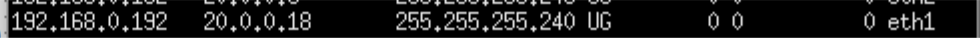
\includegraphics[width=\textwidth]{alinea_e.png}
\end{figure}

Existe uma correspondência (match) nesta entrada para pacotes enviados para o polo Galiza? E para CDN?
Caso seja essa a entrada utilizada para o encaminhamento, permitirá o funcionamento esperado do
dispositivo?
Ofereça uma explicação pela qual essa entrada é ou não utilizada.

\subsubsection{Resposta alínea e)}

As subredes Galiza e CDN têm entradas na tabela de encaminhamento com "matches" mais longos. Assim sendo, o router irá optar por essas rotas. Caso essas entradas não existissem, o tráfego não iria ser encaminhado corretamente, levando a problemas na rede.

\subsection{Alínea f)}
Os endereços utilizados pelos quatro polos são endereços públicos ou privados? E os utilizados no core da
rede/ISPs? Justifique convenientemente.

\subsubsection{Resposta alínea f)}

Os endereços são todos privados. Isto pois, fazem todos parte do "grupo" de endereços privados reservados - 192.168.0.0/24 ; 172.16.0.0/12 ; 10.0.0.8/8

\subsection{Alínea g)}
Os switches localizados em cada um dos polos têm um endereço IP atribuído? Porquê?

\subsubsection{Resposta alínea g)}

Os switches são dispositivos que operam no nível 2 (nível de dados) e são responsáveis por encaminhar o tráfego entre diferentes dispositivos conectados à rede. Ao contrário de dispositivos de nível 3, como os routers, os switches não precisam de endereços IP. Eles utilizam endereços MAC para identificar dispositivos conectados a eles e encaminhar o tráfego pela rede.
\pagebreak

\section{Parte II - Exercício 2}

Tendo feito as pazes com a mãe, D. Afonso Henriques vê-se com algum tempo livre e decide fazer remodelações no condado:

\subsection{Alínea a)}

Não estando satisfeito com a decoração do Castelo, opta por eliminar a sua rota default.
Adicione as rotas necessárias para que o Castelo continue a ter acesso a cada um dos três polos. Mostre que a
conectividade é restabelecida, assim como a tabela de encaminhamento resultante. Explicite ainda a utilidade de
uma rota default.

\subsubsection{Resposta alínea a)}

Primeiramente, apagamos a rota default do Castelo, executando o comando: ip route del default

Após isso, foram adicionadas as seguintes rotas:
\begin{figure}[h]
    \centering
    \begin{lstlisting}
> netstat -rn                                                          
Kernel IP routing table
Destination     Gateway         Genmask         Flags   MSS Window  irtt Iface
192.168.0.192   192.168.0.225   255.255.255.248 UG        0 0          0 eth0
192.168.0.200   192.168.0.225   255.255.255.248 UG        0 0          0 eth0
192.168.0.208   192.168.0.225   255.255.255.248 UG        0 0          0 eth0
192.168.0.216   192.168.0.225   255.255.255.248 UG        0 0          0 eth0
192.168.0.224   192.168.0.225   255.255.255.248 UG        0 0          0 eth0
192.168.0.224   0.0.0.0         255.255.255.248 U         0 0          0 eth0
192.168.0.232   192.168.0.225   255.255.255.248 UG        0 0          0 eth0
192.168.0.240   192.168.0.225   255.255.255.248 UG        0 0          0 eth0
192.168.0.248   192.168.0.225   255.255.255.248 UG        0 0          0 eth0
    \end{lstlisting}
\end{figure}

Por último foram feitos os testes de maneira a descobrir se este realmente estava conectado a todos os polos.

\begin{figure}[h]
    \centering
    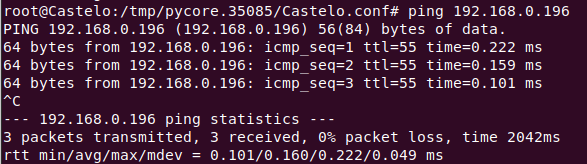
\includegraphics[width=\textwidth]{galiza2.png}
    \caption{Conexão Galiza}
\end{figure}
\pagebreak
\begin{figure}[h]
    \centering
    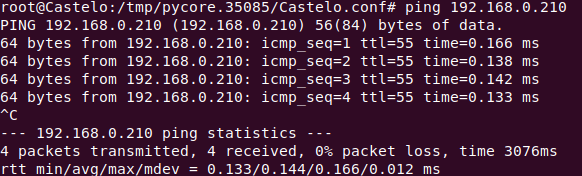
\includegraphics[width=\textwidth]{cdn-ping2.png}
    \caption{Conexão CDN}
\end{figure}

\begin{figure}[h]
    \centering
    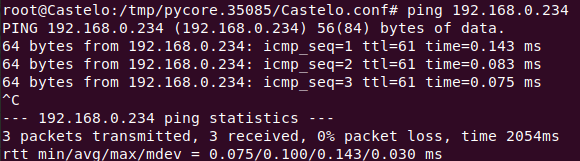
\includegraphics[width=\textwidth]{polo2.png}
    \caption{Conexão Instucional}
\end{figure}

Retirando a \emph{default} route necessitamos de reconectar o \emph{host} Castelo a todos os outros polos manualmente. Desta maneira no futuro, limitando nos a não ter a \emph{default} route, teremos problemas de conexão com futuras redes que sejam adicionadas.  
\subsection{Alínea b)}

Por modo a garantir uma posição estrategicamente mais vantajosa e ter casa de férias para relaxar entre batalhas,
ordena também a construção de um segundo Castelo, em Braga. Não tendo qualquer queixa do serviço prestado,
recorre novamente aos serviços do ISP ReiDaNet para ter acesso à rede no segundo Castelo. O ISP atribuiu-lhe
o endereço de rede IP 172.16.XX.128/26 em que XX corresponde ao seu número de grupo (PLXX). Defina um
esquema de endereçamento que permita o estabelecimento de pelo menos 3 redes e que garanta que cada uma
destas possa ter 10 ou mais hosts. Assuma que todos os endereços de sub-redes são utilizáveis.

\subsubsection{Resposta alínea b)}

Para o endereço IP 172.16.12.128/26 temos um total de 64 endereços, como queremos pelo menos 3 redes precisamos de pelo menos 2 bits de maneira a representá-las, assim a máscara deixará de ser /26 e passará a ser /28, e por consequência de utilizarmos 2 bits acabamos com 4 redes. Dividindo o número de endereços por cada rede: \[64/4 = 16\] Concluímos que cada rede terá 16 endereços, 14 usáveis.

\begin{itemize}
    \item 1ª Rede: 172.16.12.128/28
    \begin{description}
        \item[Range:] 172.16.12.129 - 172.16.12.142    
        \item[Broadcast:] 172.16.12.143
    \end{description}
    \item 2ª Rede: 172.16.12.144/28
    \begin{description}
        \item[Range:] 172.16.12.145 - 172.16.12.158      
        \item[Broadcast:] 172.16.12.159 
    \end{description}
    \item 3ª Rede: 172.16.12.160/28
    \begin{description}
        \item[Range:] 172.16.12.161 - 172.16.12.173   
        \item[Broadcast:] 172.16.12.175
    \end{description}
    \bigskip
    \item 4ª Rede: 172.16.12.176/28
    \begin{description}
        \item[Range:] 172.16.12.177 - 172.16.12.190    
        \item[Broadcast:] 172.16.12.191
    \end{description}
\end{itemize}

\subsection{Alínea c)}

Ligue um novo host diretamente ao router ReiDaNet. Associe-lhe um endereço, à sua escolha, pertencente a uma
sub-rede disponível das criadas na alínea anterior (garanta que a interface do router ReiDaNet utiliza o primeiro
endereço da sub-rede escolhida). Verifique que tem conectividade com os diferentes polos.
Existe algum host com o qual não seja possível comunicar? Porquê?

\subsubsection{Resposta alínea c)}

\begin{figure}[h]
    \centering
    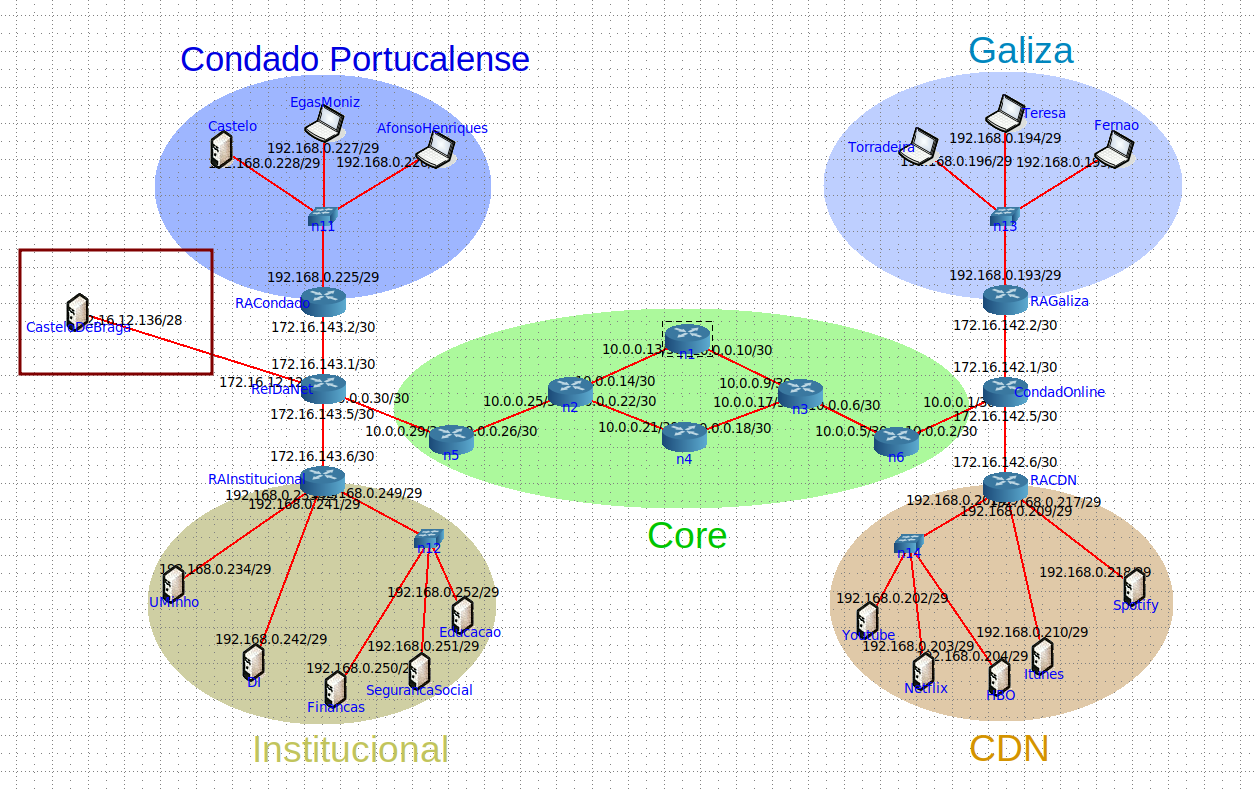
\includegraphics[width=\textwidth]{topologia2-c.png}
    \caption{Topologia do exercício}
\end{figure}

Ligamos um host ao ReiDaNet, associando-lhe o endereço 172.16.12.129/28.
Em baixo, segue a demonstração da ligação, com sucesso, a todos os polos.

\begin{figure}[h]
    \centering
    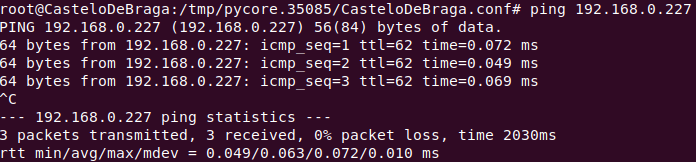
\includegraphics[width=\textwidth]{portucalense_c.png}
    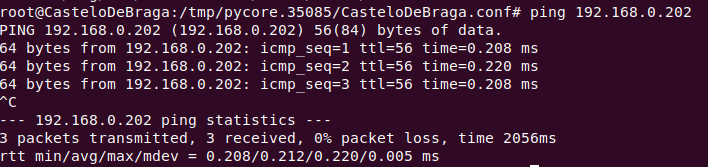
\includegraphics[width=\textwidth]{cdn_c.png}
    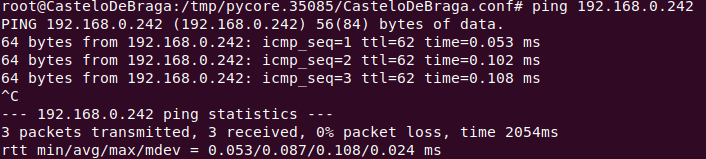
\includegraphics[width=\textwidth]{inst_c.png}
    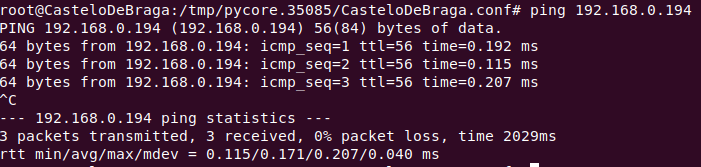
\includegraphics[width=\textwidth]{galiza_c.png}
    \caption{Conexão, respetivamente, com o Condado, o CDN, o Instituto e a Galiza}
\end{figure}


\pagebreak

\section{Parte II - Exercício 3}

Ao planear um novo ataque, D. Afonso Henriques constata que o seu exército não só perde bastante tempo a decidir
que direção tomar a cada salto como, por vezes, inclusivamente se perde.

\subsection{Alínea a)}

De modo a facilitar a travessia, elimine as rotas referentes a Galiza e CDN no dispositivo n6 e defina um
esquema de sumarização de rotas (Supernetting) que permita o uso de apenas uma rota para ambos os
polos. Confirme que a conectividade é mantida

\subsubsection{Resposta alínea a)}

Executando os comandos no dispositivo n6:
\begin{lstlisting}
> ip route del 192.168.0.192/29
> ip route del 192.168.0.200/29
> ip route del 192.168.0.208/29
> ip route del 192.168.0.216/29
\end{lstlisting}
Conseguimos remover as rotas referentes a Galiza e CDN.
\bigskip

Temos agora que encontrar o IP novo que irá agregar todos os IPs anteriores num só.

Listando-os todos e convertendo para binário o padrão que é incomum nas subredes:
\begin{lstlisting}
192.168.0.11000000/29
192.168.0.11001000/29
192.168.0.11010000/29
192.168.0.11011000/29
\end{lstlisting}

Determinar onde a primeira mudança ocorre:
\begin{lstlisting}
192.168.0.110|00|000/29
192.168.0.110|01|000/29
192.168.0.110|10|000/29
192.168.0.110|11|000/29
\end{lstlisting}

Converter IP:
\begin{lstlisting}
192.168.0.11000000/27
\end{lstlisting}
 ou seja 
 \begin{lstlisting}
192.168.0.192/27
\end{lstlisting}

Para finalizar, basta adicionar uma rota no IP 192.168.0.192/27 via 10.0.0.1, e então conseguimos fazer com que exista apenas uma rota para ambos os polos.
 \begin{lstlisting}
> ip route add 192.168.0.192/27 via 10.0.0.1
\end{lstlisting}

\begin{figure}[h]
    \centering
    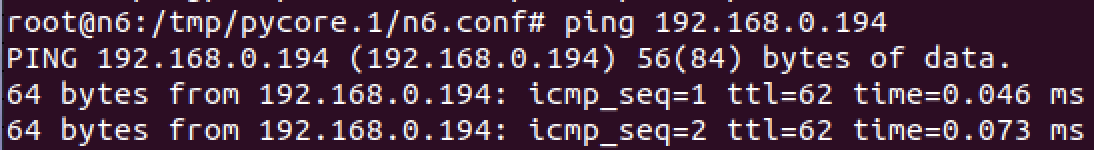
\includegraphics[width=\textwidth]{galiza3.png}
    \caption{Conectividade a Teresa, Galiza.}
\end{figure}
\begin{figure}[h]
    \centering
    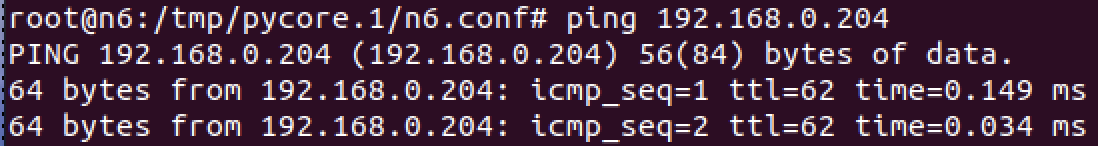
\includegraphics[width=\textwidth]{cdn-hbo3.png}
    \caption{Conectividade a HBO, CDN.}
\end{figure}
\begin{figure}[h]
    \centering
    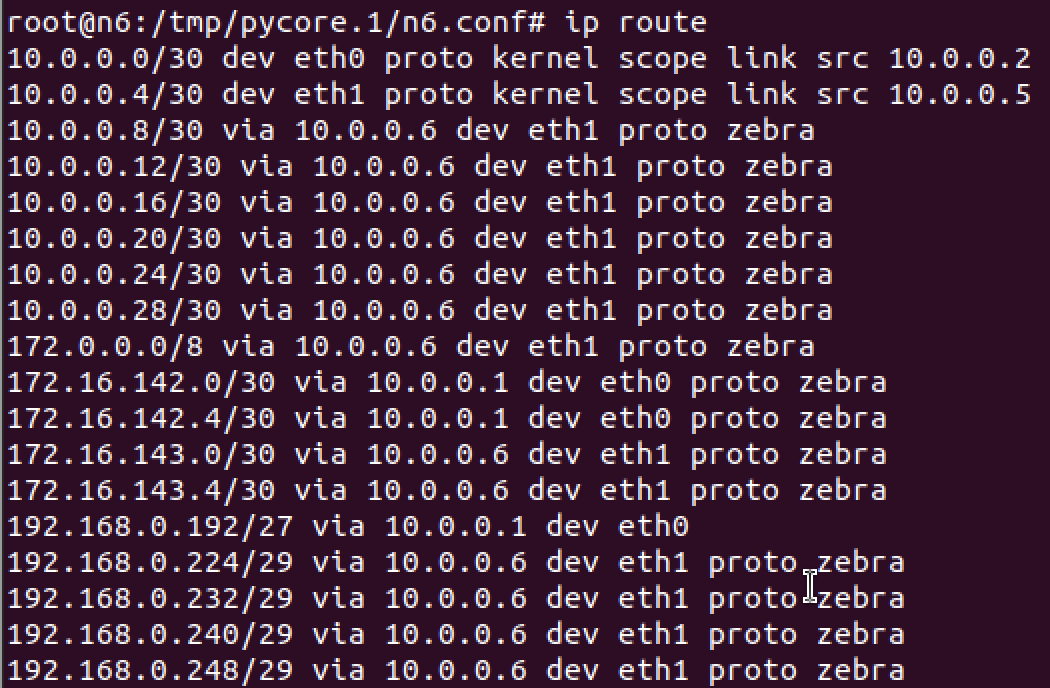
\includegraphics[width=\textwidth]{route-table-3.png}
    \caption{Route Table}
\end{figure}
\pagebreak

\subsection{Alínea b)}

Repita o processo descrito na alínea anterior para CondadoPortucalense e Institucional, também no dispositivo n6

\subsubsection{Resposta alínea b)}

 Fazendo o mesmo processo da alínea anterior só que para os IPs do Condado e do Institucional:

 \begin{lstlisting}
> ip route del 192.168.0.224/29
> ip route del 192.168.0.232/29
> ip route del 192.168.0.240/29
> ip route del 192.168.0.248/29
\end{lstlisting}

Executamos estes comandos para eliminar as rotas presentes.
Aplicando o mesmo algoritmo para descobrir o novo IP da rota temos como resultado: 
\begin{lstlisting}
192.168.0.224/27
\end{lstlisting}
 e então basta adicioná-lo como nova rota:
 \begin{lstlisting}
> ip route add 192.168.0.224/27 via 10.0.0.6
\end{lstlisting}
\pagebreak
\begin{figure}[h]
    \centering
    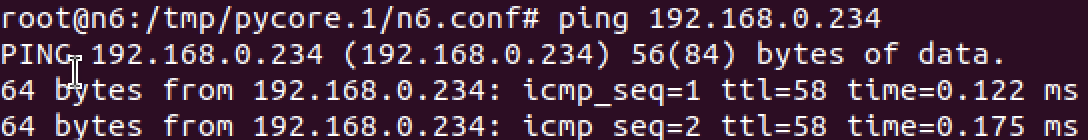
\includegraphics[width=\textwidth]{uminho-inst.png}
    \caption{Dispositivo UMinho Instituto}
\end{figure}

\begin{figure}[h]
    \centering
    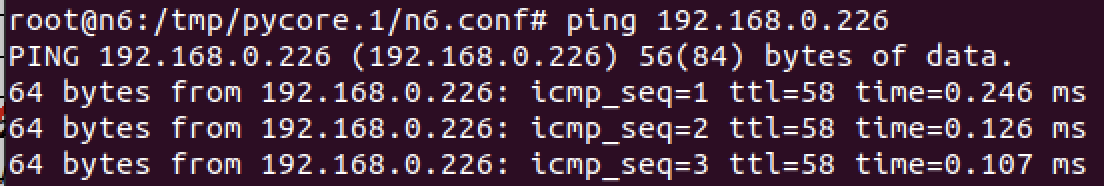
\includegraphics[width=\textwidth]{ah-condado.png}
    \caption{Dispositivo Afonso Henriques Condado}
\end{figure}

\begin{figure}[h]
    \centering
    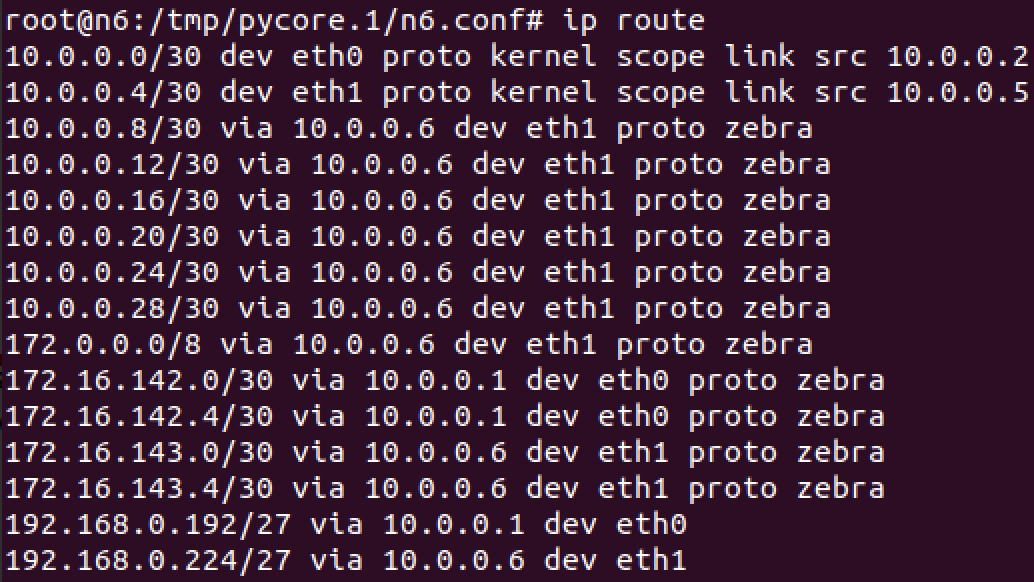
\includegraphics[width=\textwidth]{iptable.png}
    \caption{Route Table}
\end{figure}

\subsection{Alínea c)}

Comente os aspetos positivos e negativos do uso do \emph{Supernetting}.

\subsubsection{Resposta alínea c)}
Aspetos positivos:
\begin{itemize}
    \item O tamanho da lista das rotas é menor, poupando tempo no CPU e memória.
    \item Abstrai topologias de outros routers, fazendo com que, quando essas alteradas, as rotas do nosso router não precisem de ser alteradas.
\end{itemize}

Aspetos negativos:
\begin{itemize}
    \item Quanto maior a gama de IPs que uma entrada nas rotas do nosso router cobre, mais IPs podem não estar a ser usados, sendo assim desperdiçados
\end{itemize}











\end{document}
